\documentclass[class=extarticle,14pt,tikz,border=12pt]{standalone}

% Poster typography
\usepackage[T1]{fontenc}
\usepackage{tgheros}
\usepackage[final]{microtype}
\renewcommand{\familydefault}{\sfdefault}

\usepackage{xcolor}
\usepackage{amsmath}
\usepackage{relsize}
\usepackage{tikz}
\usetikzlibrary{positioning,shadows.blur}

% ---- Palette ----
\definecolor{farsun}{HTML}{1F77B4}   % 2025
\definecolor{plum}{HTML}{9467BD}     % 2026
\definecolor{rob}{HTML}{2CA02C}      % 2026--2027
\definecolor{silso}{HTML}{FF7F0E}    % 2027
\definecolor{slate}{HTML}{1F2937}    % neutral
\colorlet{greenShadeA}{rob!75!white}
\colorlet{greenShadeB}{rob}
\colorlet{greenShadeC}{rob!80!black}

% ---- Text helpers ----
\newcommand{\CardTitle}[1]{{\bfseries\LARGE #1}}
\newcommand{\CardText}[1]{{\bfseries\large #1}}
\newcommand{\SN}{\ensuremath{\mathlarger{\boldsymbol{S}_{\!N}}}}
\newcommand{\GN}{\ensuremath{\mathlarger{\boldsymbol{G}_{\!N}}}}

% ---- Styles ----
\tikzset{
  every node/.style={font=\bfseries, text=slate},
  pinup/.style={densely dashed, line width=1.1pt, draw=#1, opacity=0.95},
  % colored card (arg1=color, arg2=width)
  cardC/.style 2 args={
    rectangle, rounded corners=3mm, align=left,
    draw=#1!35!black, line width=0.6pt, fill=#1!92,
    text=white, inner sep=8pt, blur shadow,
    text width=#2
  }
}

\begin{document}
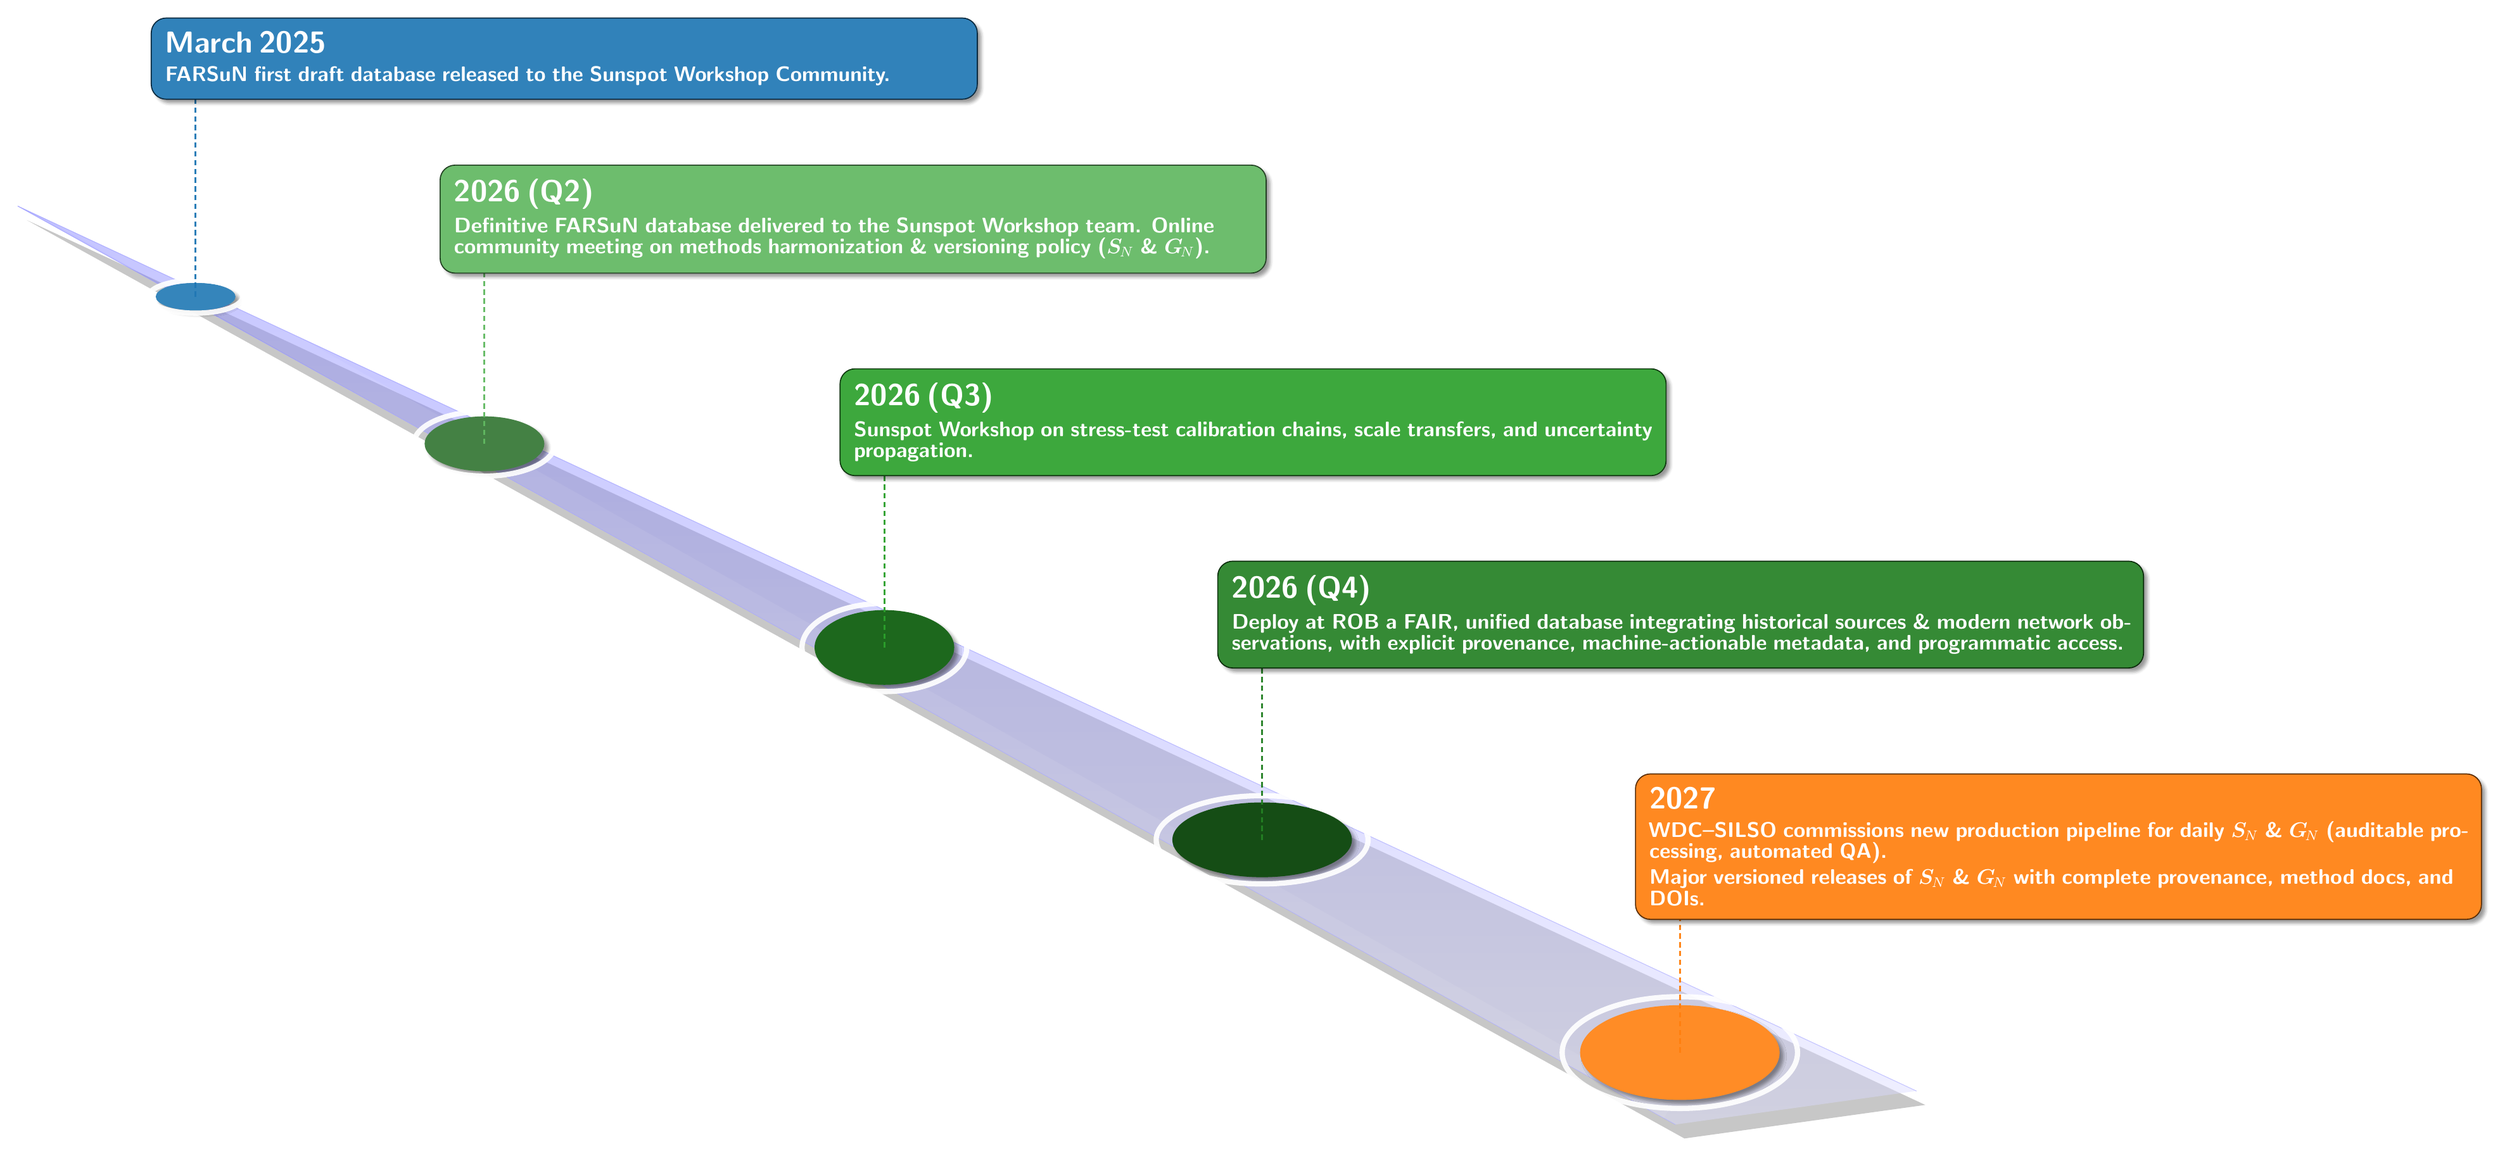
\begin{tikzpicture}[x=1cm,y=1cm]

% =========================
% ROAD (longer, clean, with depth)
% =========================
\def\angUp{-29}
\def\angLo{-25}
\def\lenUp{38.0}
\def\lenLo{42.0}
\coordinate (start) at (-14,1.4);
\coordinate (endA)  at ($(start)+(\angUp:\lenUp)$);
\coordinate (endB)  at ($(start)+(\angLo:\lenLo)$);

% shadow
\begin{scope}[opacity=0.22]
  \fill[black] ($(start)+(0.18,-0.28)$) -- ($(endA)+(0.18,-0.28)$)
               -- ($(endB)+(0.18,-0.28)$) -- cycle;
\end{scope}

% edges
\draw[line join=round,line cap=round,opacity=0.65,
      top color=blue!10,bottom color=blue!60, draw=blue!35]
      (start) -- (endA);
\draw[line join=round,line cap=round,opacity=0.65,
      top color=blue!10,bottom color=blue!60, draw=blue!35]
      (start) -- (endB);

% fill + highlight
\begin{scope}
  \path[clip] (start) -- (endA) -- (endB) -- cycle;
  \shade[bottom color=blue!10, top color=blue!60, opacity=0.45]
        ($(start)+(-1,2)$) rectangle ($(endB)+(1,-2)$);
  \draw[white, line width=12pt, opacity=0.08]
        ($(start)+(0.2,0.18)$) -- ($(endA)+(-0.2,0.18)$);
\end{scope}

% =========================
% MILESTONES (positions along the road)
% =========================
% distances along road (cm) – tweak to change spacing
\def\dA{ 4.0}  % 2025
\def\dB{ 10.5}  % 2026 (delivery)
\def\dC{19.5}  % 2026 (meeting)
\def\dD{28.}  % 2026–2027 (FAIR DB)
\def\dE{37.4}  % 2027 (ops/releases)

\pgfmathsetmacro{\midang}{(\angUp+\angLo)/2}
\coordinate (P25)  at ($(start)+(\midang:\dA)$);
\coordinate (P26a) at ($(start)+(\midang:\dB)$);
\coordinate (P26b) at ($(start)+(\midang:\dC)$);
\coordinate (P267) at ($(start)+(\midang:\dD)$);
\coordinate (P27)  at ($(start)+(\midang:\dE)$);

% discs + rims (for nice perspective)
\foreach \P/\xr/\yr/\clr in {
  P25/8mm/2.8mm/farsun!90,
  P26a/12mm/5.5mm/greenShadeA!70!black,
  P26b/14mm/7.5mm/greenShadeB!65!black,
  P267/18mm/7.5mm/greenShadeC!60!black,
  P27/20mm/9.5mm/silso!90
}{
  \path[blur shadow, draw=none, fill=\clr] (\P) ellipse [x radius=\xr, y radius=\yr];
  \draw[white, line width=3pt, opacity=0.92] (\P) ellipse [x radius=1.18*\xr, y radius=1.18*\yr];
}

% =========================
% PINS that connect straight into the cards
% =========================
\def\pinH{4.8} % vertical pin height
\coordinate (T25)  at ($(P25)+(0,\pinH)$);
\coordinate (T26a) at ($(P26a)+(0,\pinH)$);
\coordinate (T26b) at ($(P26b)+(0,\pinH)$);
\coordinate (T267) at ($(P267)+(0,\pinH)$);
\coordinate (T27)  at ($(P27)+(0,\pinH)$);

\draw[pinup=farsun] (P25)  -- (T25);
\draw[pinup=greenShadeA] (P26a) -- (T26a);
\draw[pinup=greenShadeB] (P26b) -- (T26b);
\draw[pinup=greenShadeC] (P267) -- (T267);
\draw[pinup=silso]  (P27)  -- (T27);

% =========================
% CARDS REPLACING YEAR LABELS (placed right of pin top)
% =========================
\def\xoff{-0.9}  % how far to the right of the pin top
\def\yoff{0.8} % slight drop below the pin top

\node[cardC={farsun}{16.0cm}, anchor=north west]
  (C25)  at ($(T25)+(\xoff,\yoff)$)   {\CardTitle{March 2025}\\[4pt]
  \CardText{FARSuN \emph{first draft database} released to the Sunspot Workshop Community.}};

\node[cardC={greenShadeA}{16.0cm}, anchor=north west]
  (C26a) at ($(T26a)+(\xoff,\yoff)$)  {\CardTitle{2026 (Q2)} \\[4pt]
  \CardText{\textit{Definitive} FARSuN database delivered to the Sunspot Workshop team. Online community meeting on methods harmonization \& versioning policy (\SN{} \& \GN{}).}};

\node[cardC={greenShadeB}{16.0cm}, anchor=north west]
  (C26b) at ($(T26b)+(\xoff,\yoff)$)  {\CardTitle{2026 (Q3) }\\[4pt]
  \CardText{Sunspot Workshop on stress-test calibration chains, scale transfers, and uncertainty propagation.}};

\node[cardC={greenShadeC}{18.0cm}, anchor=north west]
  (C267) at ($(T267)+(\xoff,\yoff)$) {\CardTitle{2026 (Q4)}\\[4pt]
  \CardText{Deploy at ROB a FAIR, unified database integrating historical sources \& modern network observations, with explicit provenance, machine-actionable metadata, and programmatic access.}};

\node[cardC={silso}{16.4cm}, anchor=north west]
  (C27)  at ($(T27)+(\xoff,\yoff)$)   {\CardTitle{2027}\\[4pt]
  \CardText{WDC--SILSO commissions new production pipeline for daily \SN{} \& \GN{} (auditable processing, automated QA).}\\[3pt]
  \CardText{Major versioned releases of \SN{} \& \GN{} with complete provenance, method docs, and DOIs.}};

\end{tikzpicture}
\end{document}
